\section{Formationen}
Um sich durch das Gelände zu bewegen verwendet man Formationen. Diese können für die Trupp von Vorteil sein oder gewisse Nachteile haben. Deshalb sollten sie jederzeit dem Gelände, sowie erwarteten oder bekannten Situationen angepasst werden. Die Formationen die im TTT Verwendung finden sind der \textit{Stack}, die \textit{Kolonne} und die \textit{Schützenkette}. 

\subsection{Der Stack}
Der Stack ist die Sammelformation vor dem Abmarsch und als Bewegungsformation beim Einstieg in Fahrzeuge. Zudem dient er als Formation für den direkten Zugriff in Räume (siehe dazu CQB, \autoref{CQB}). Grundsätzlich wird der Stack in den klassischen (engen) <<Stack>> und <<Stack weit>> unterteilt. Beim <<Stack weit>> werden die Abstände lediglich erweitert.
\begin{figure}[h]
	\centering
	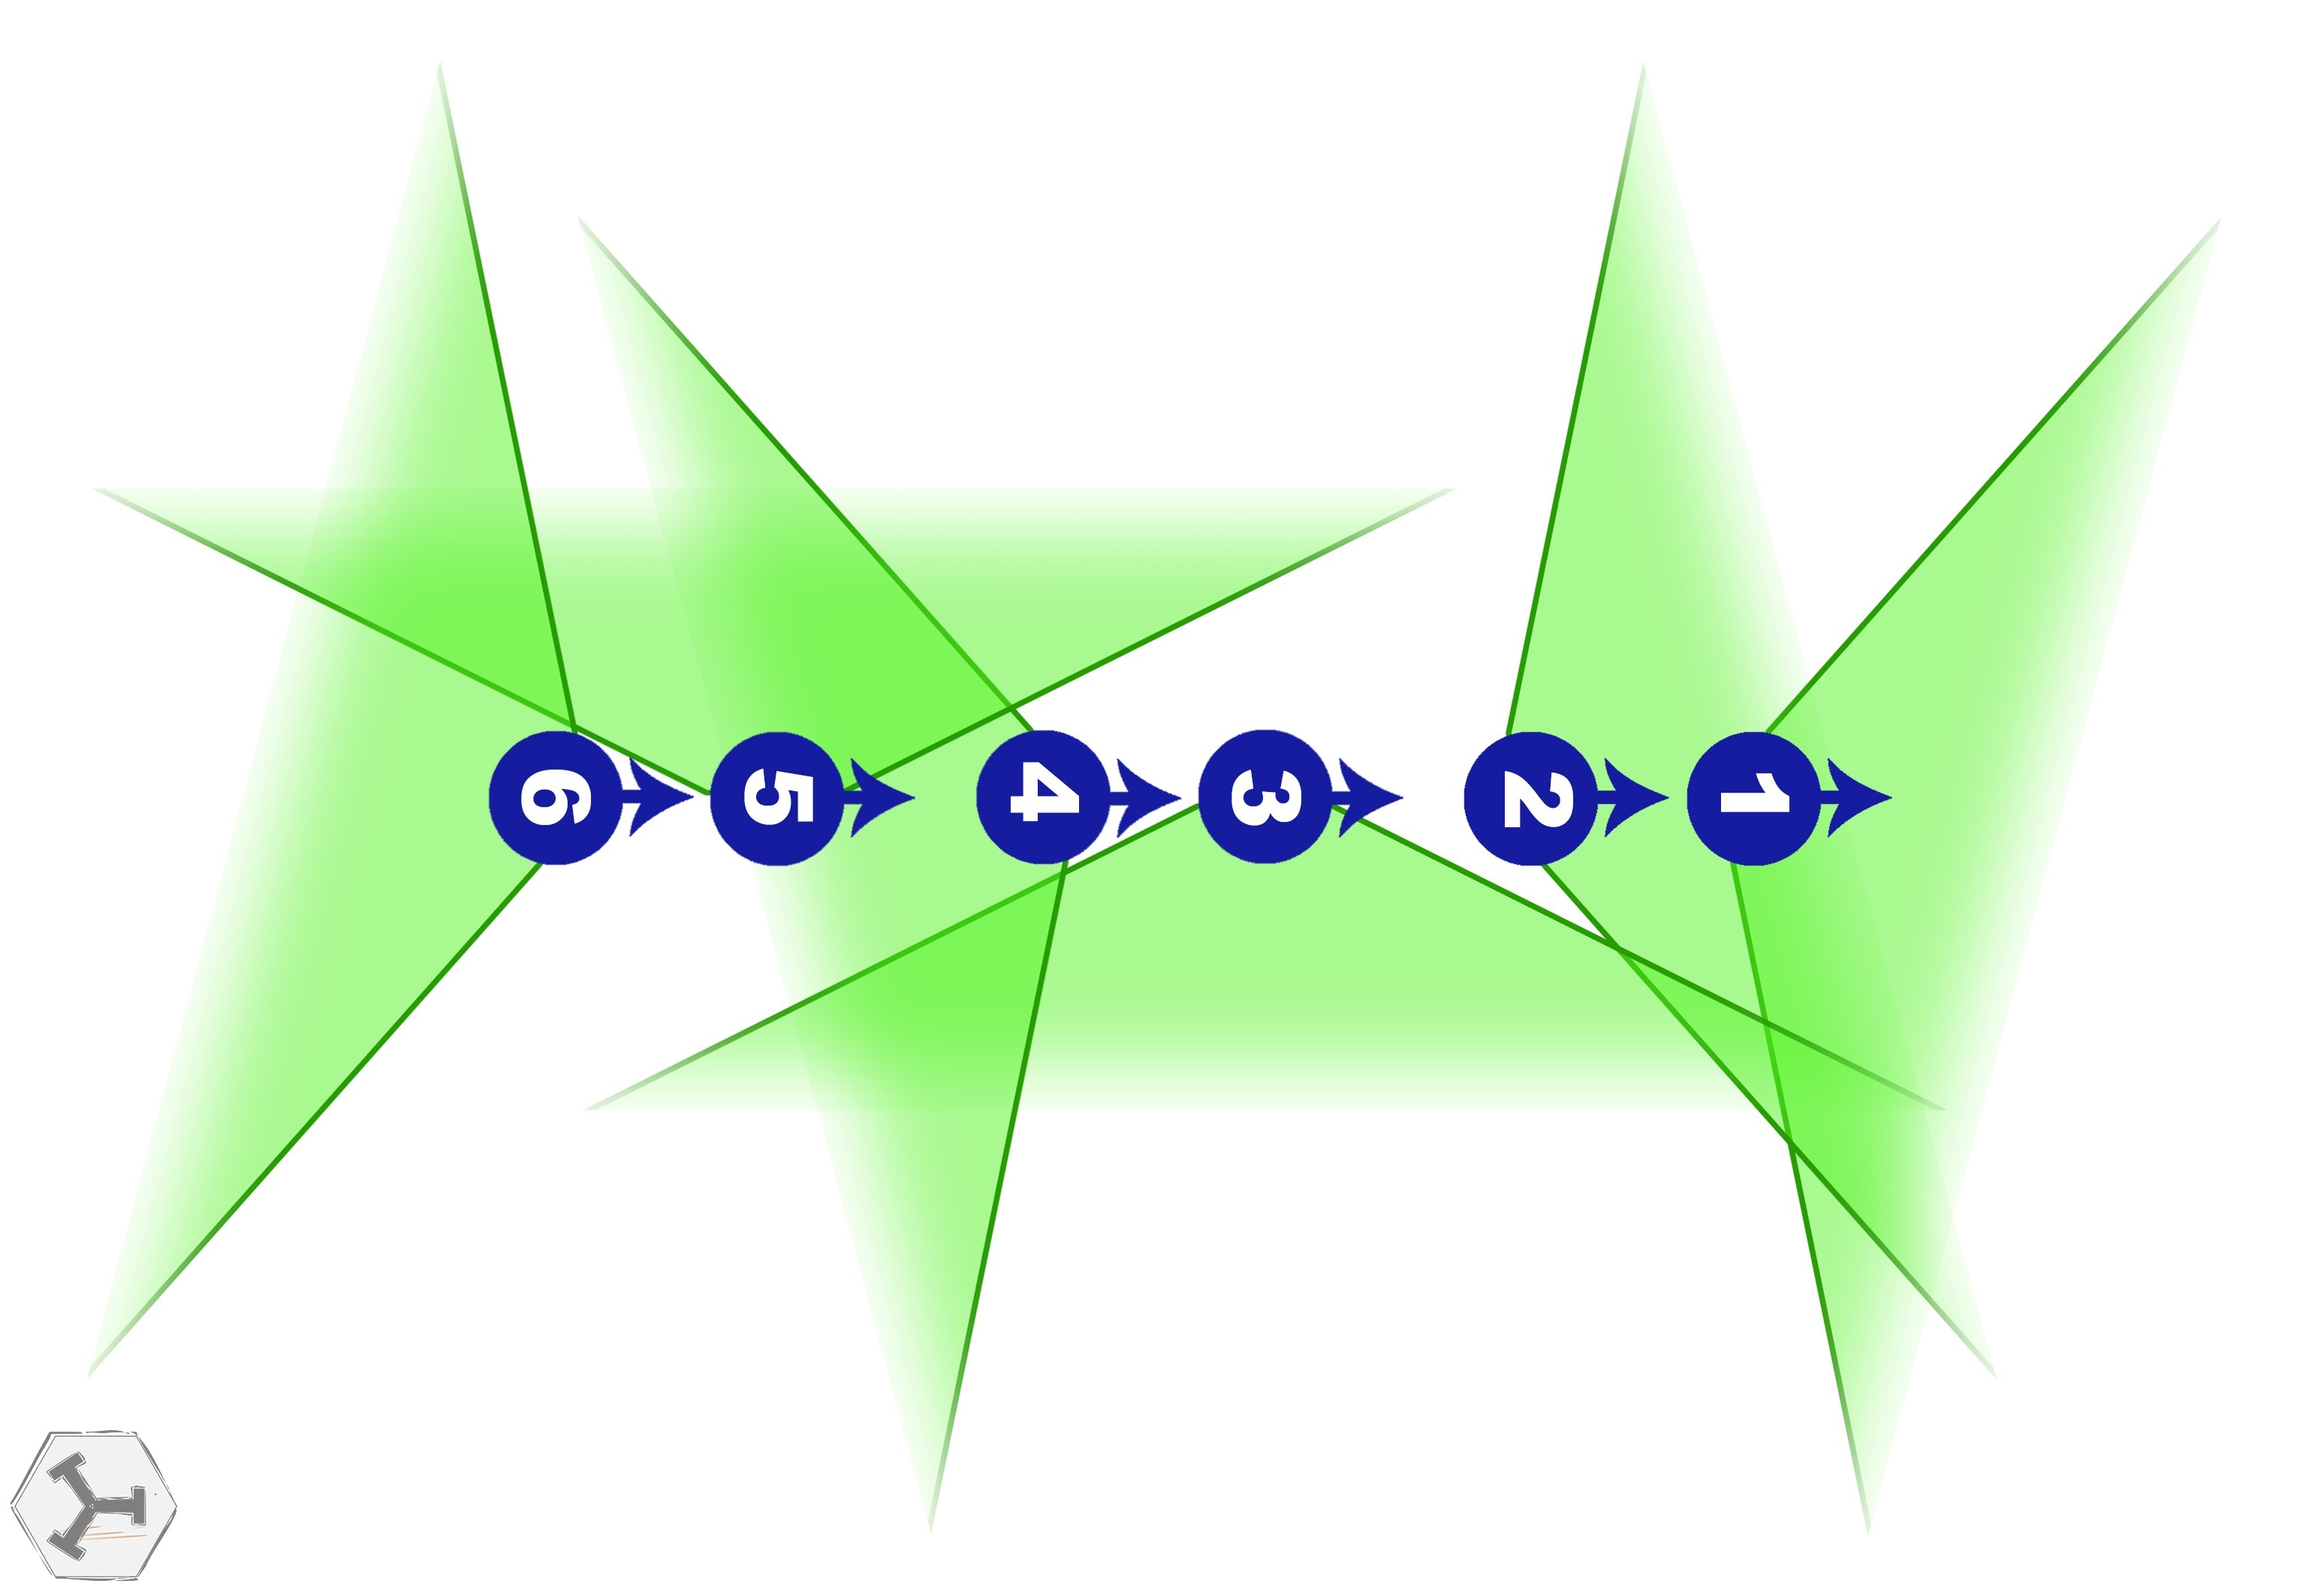
\includegraphics[width=0.7\linewidth]{./img/grundlagen/formationen/stack_6mann}
	\caption{Stack 6 Mann}
\end{figure}\\

\subsection{Die Kolonne}\label{Kolonne}
Die Kolonne dient als Formation im offenen Gelände und ist die Standardformation für den Marsch. Hierbei muss man zwischen einer Besonderheit im \ac{TTT} der Buddy"=Kolonne und der klassischen Kolonne unterscheiden. Die Buddy"=Kolonne garantiert, dass beispielsweise MG-Schütze und MG-Assistent immer zusammenbleiben. Zudem verringert sie die Ausfallzahl, da sich Buddies besser gegenseitig unterstützen können. Im Gegenzug ist die klassische Kolonne weniger anfällig für Sprengsätze und Beschuss. Die Abstände zwischen den Teams sollten etwa 20\,m betragen.
\begin{figure}[h]
	\centering
	\subfigure[Kolonne]{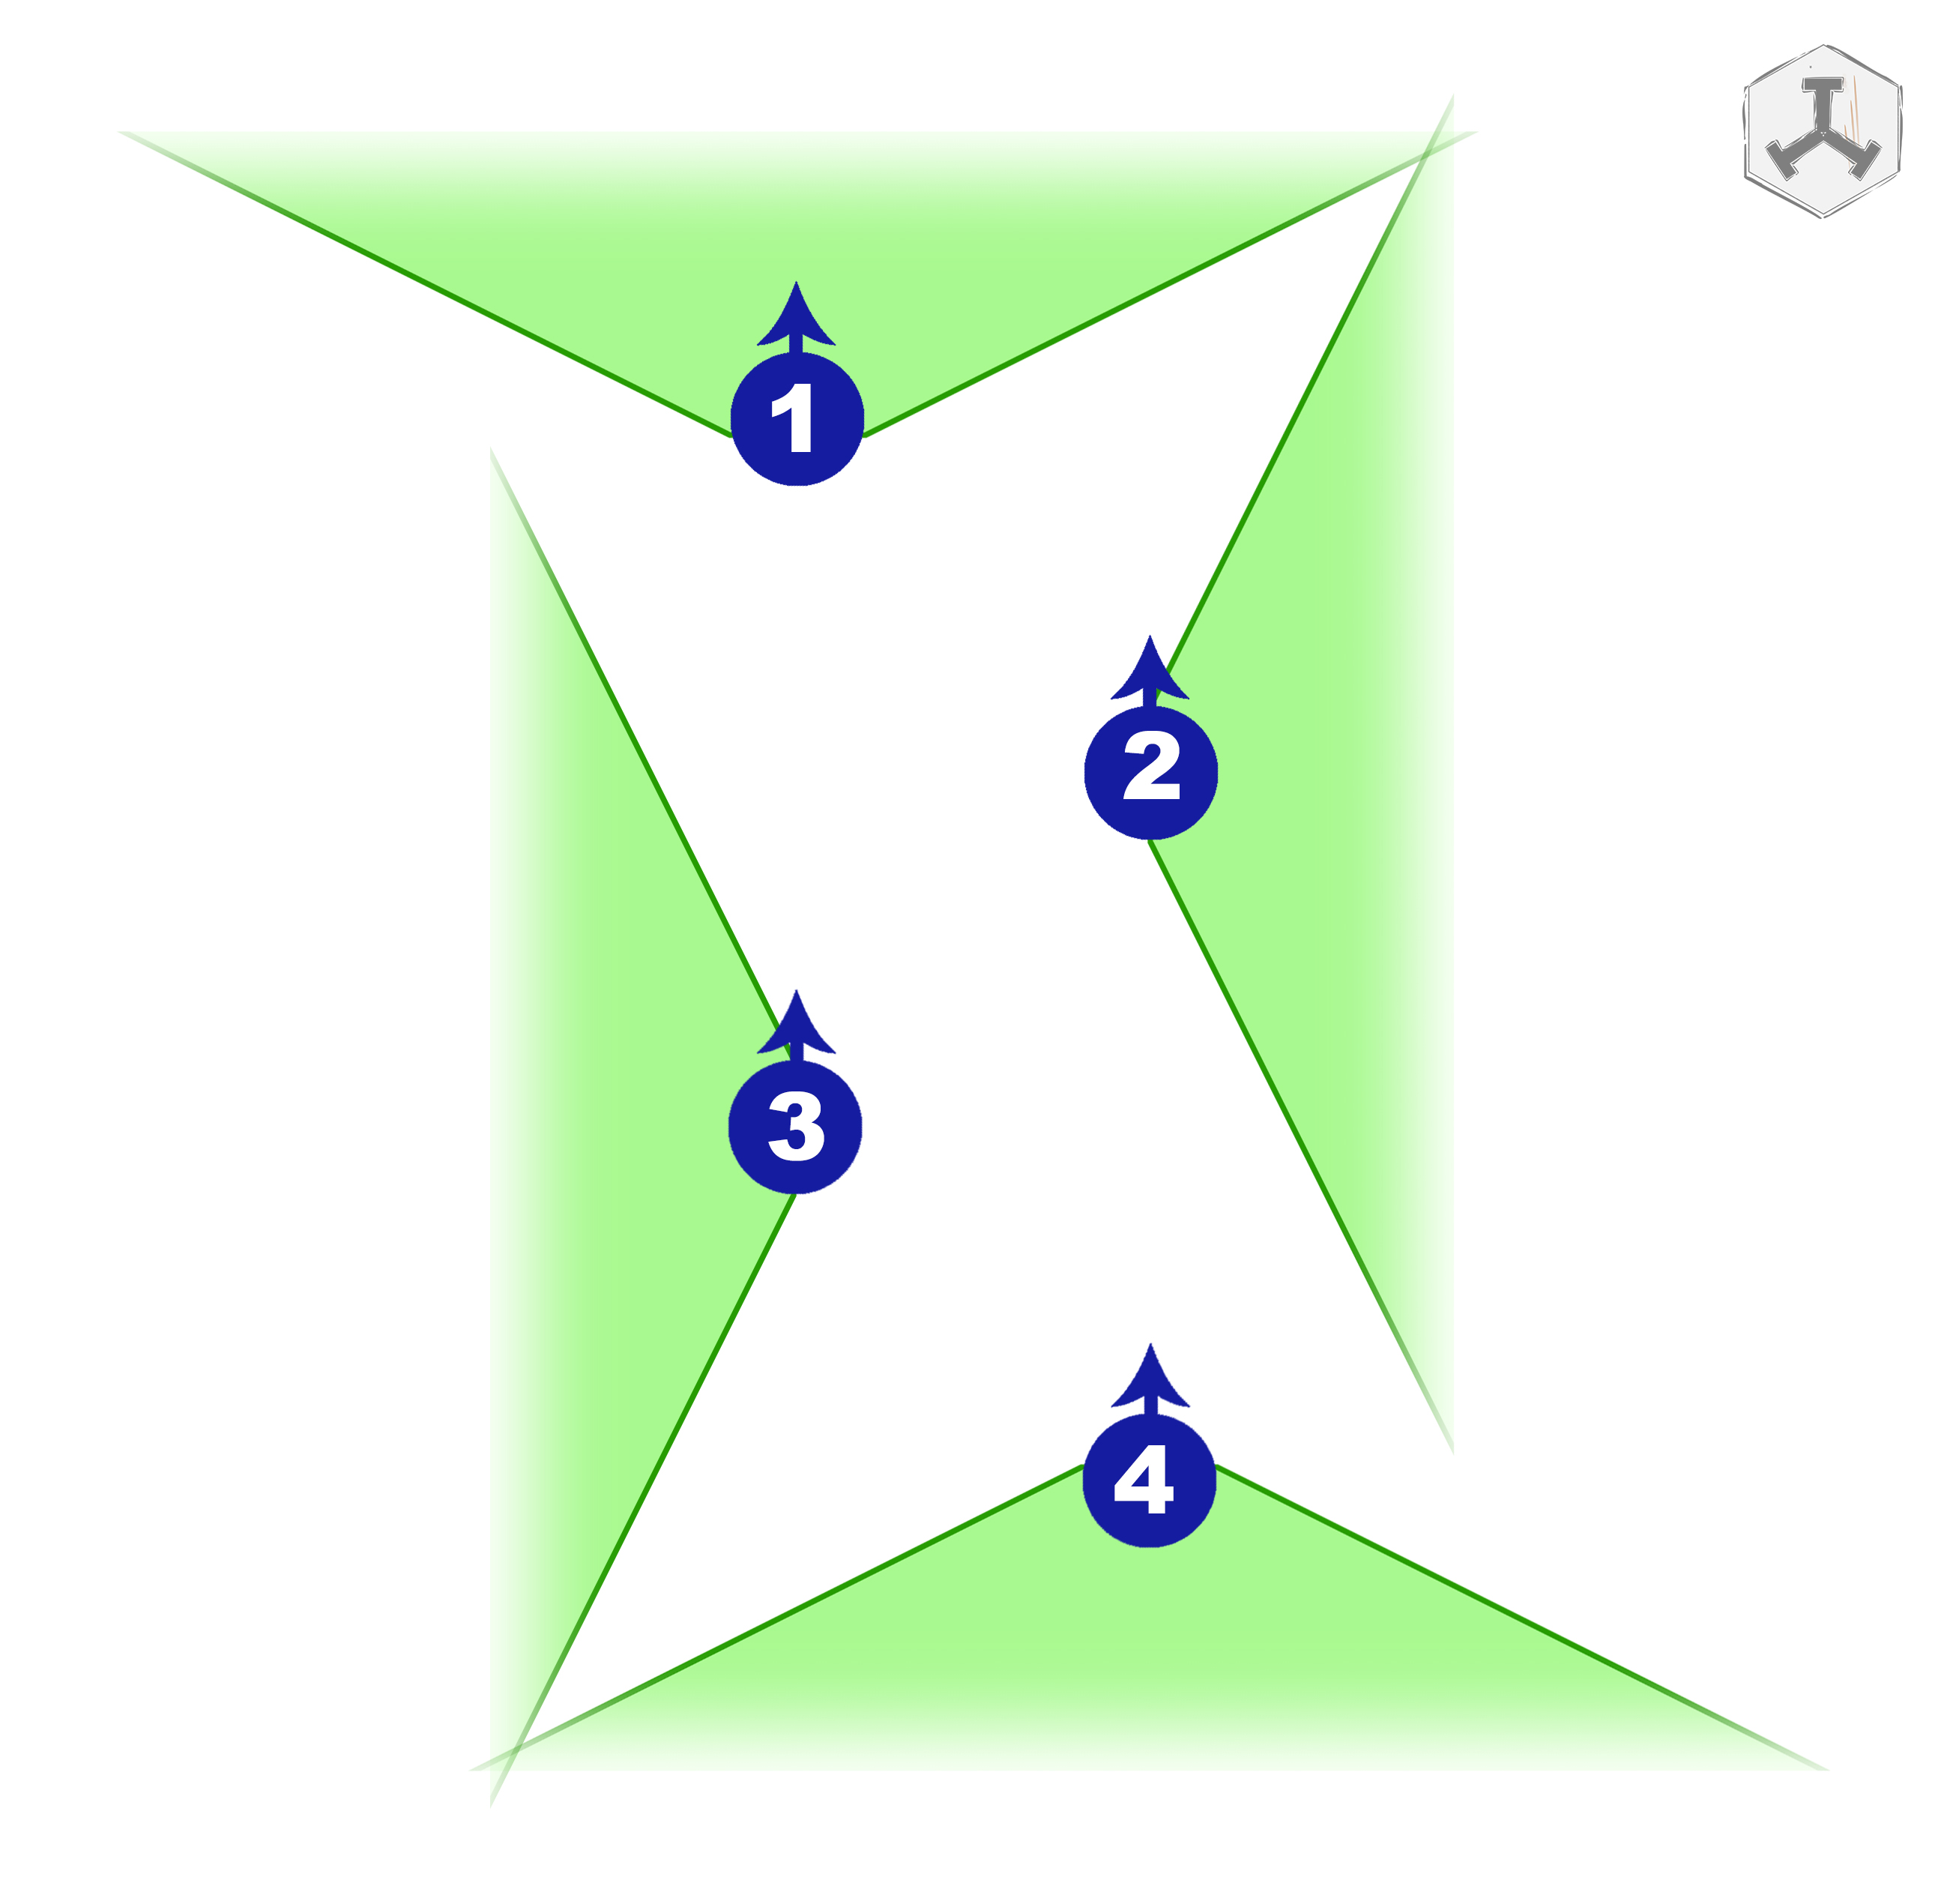
\includegraphics[width=0.49\linewidth]{./img/grundlagen/formationen/kolonne_4mann}}
	\subfigure[Buddy-Kolonne]{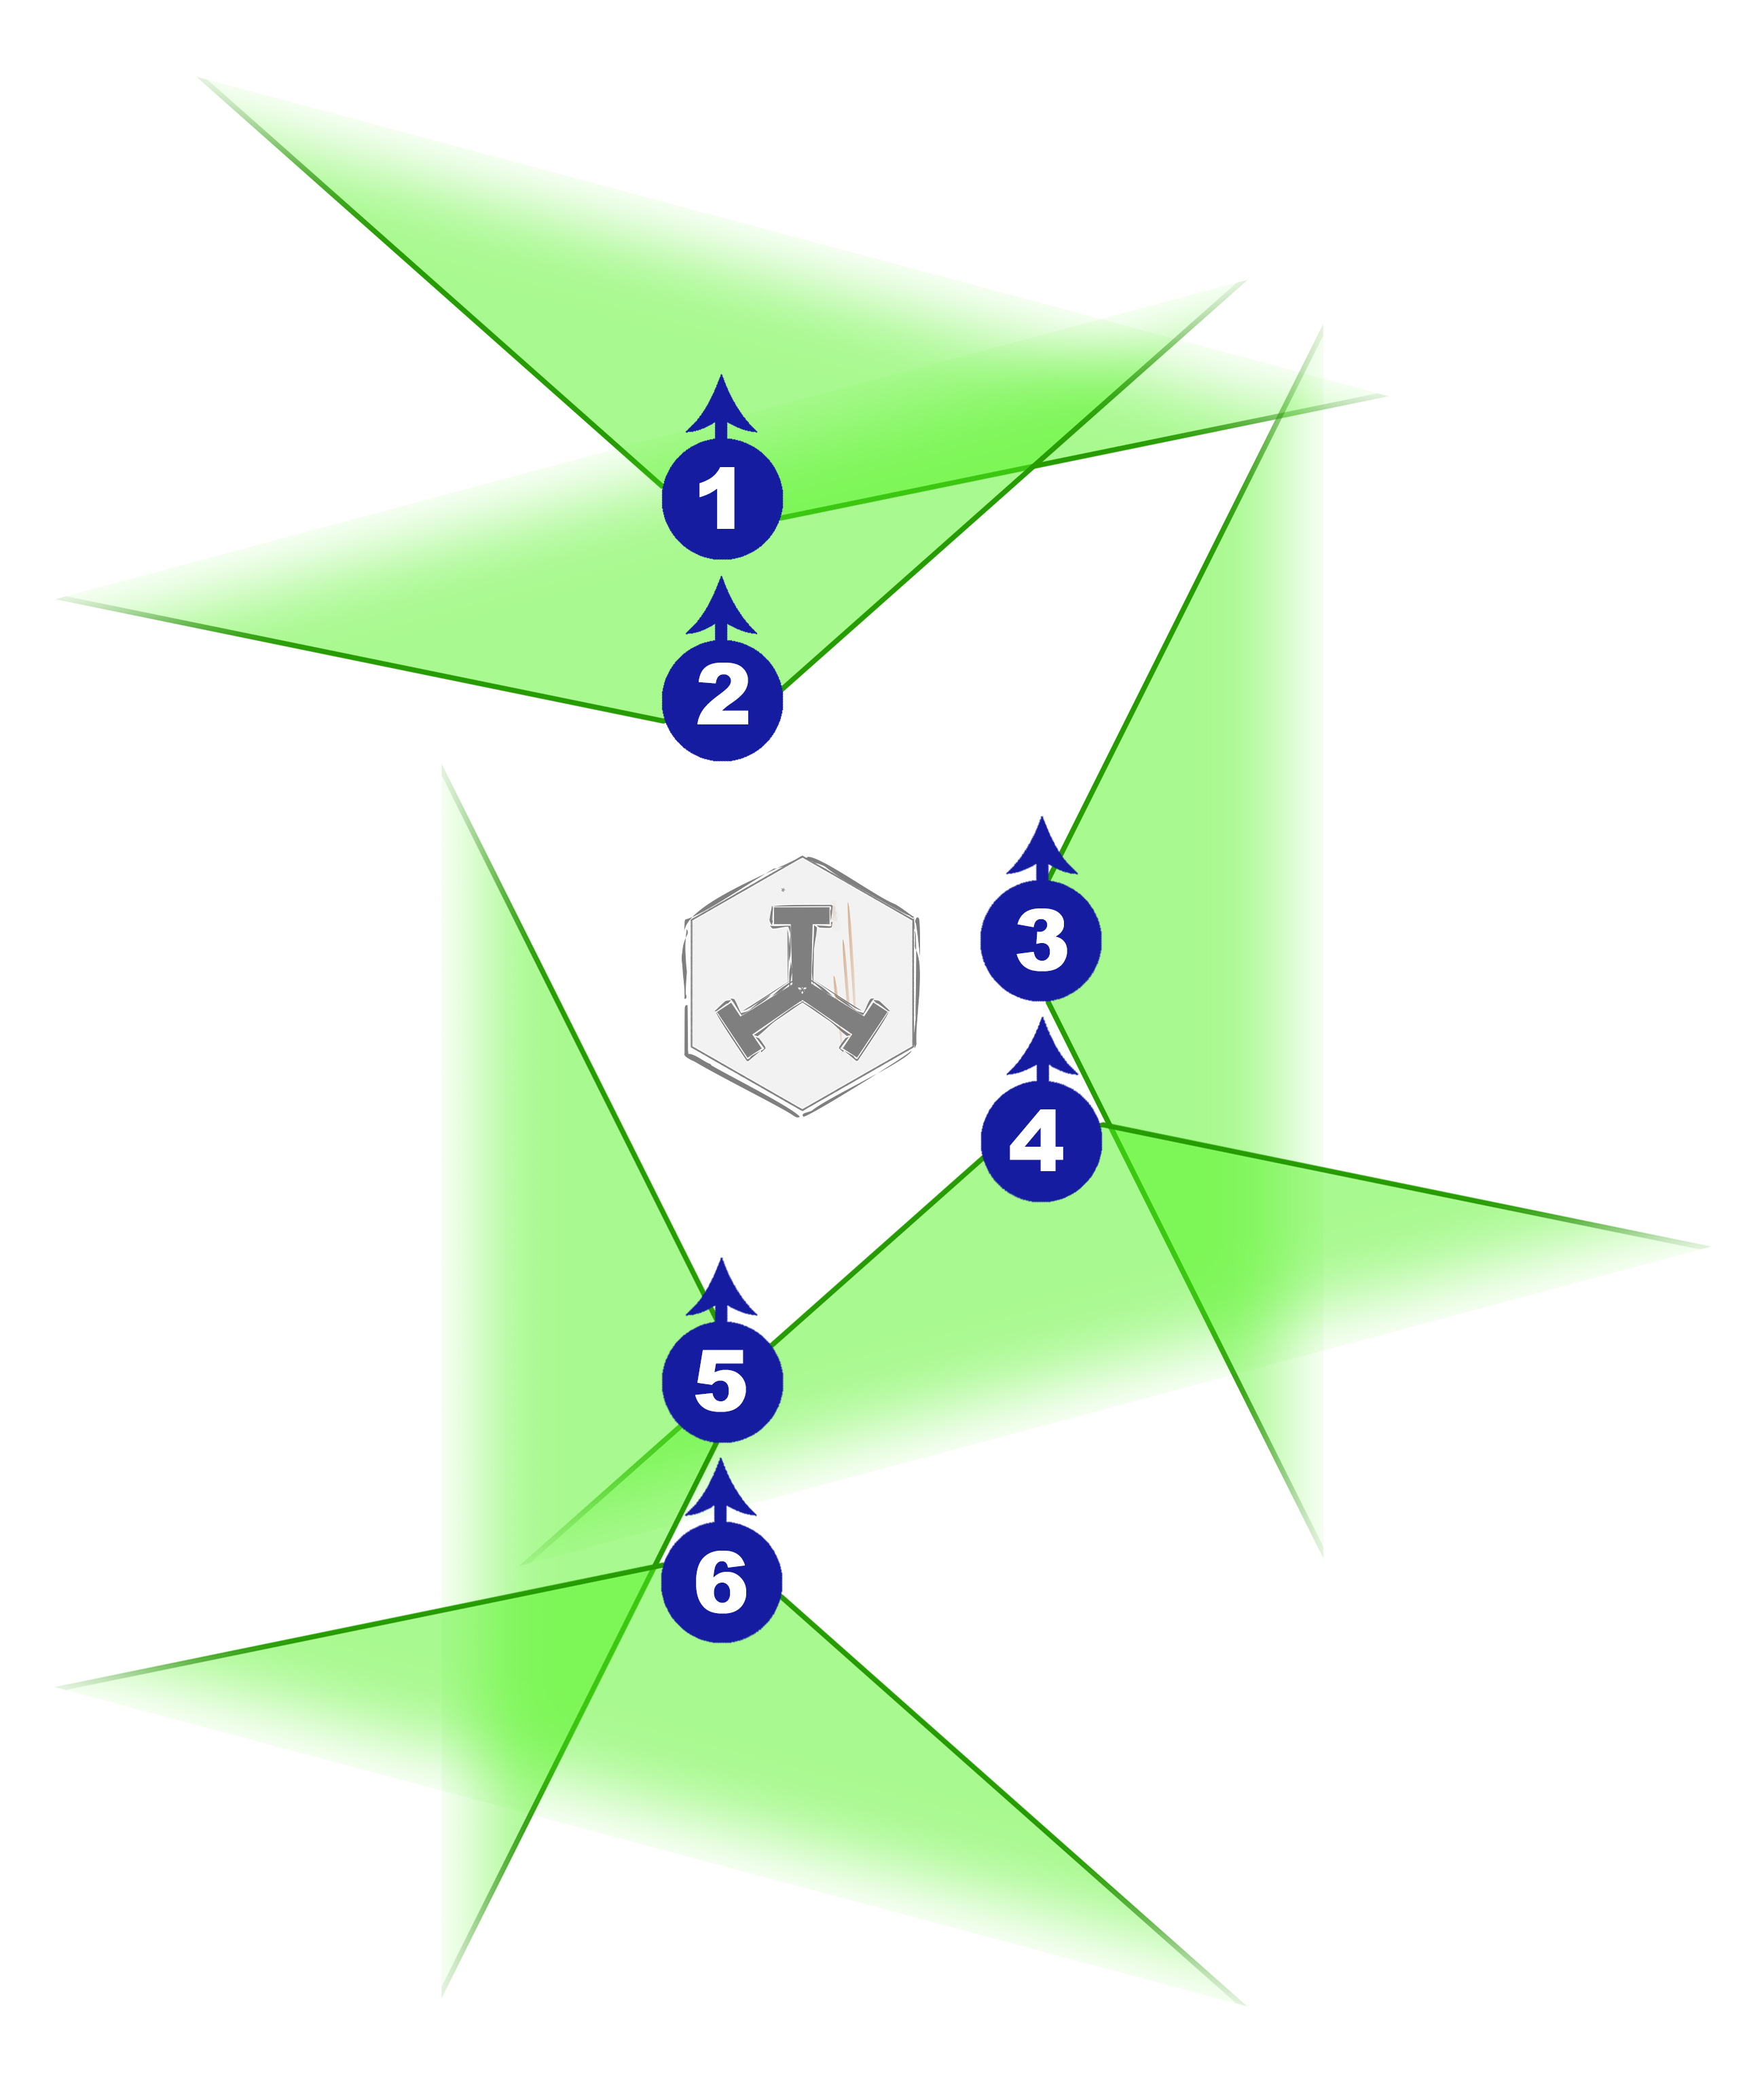
\includegraphics[width=0.49\linewidth]{./img/grundlagen/formationen/kolonne_6mann}}
	\label{fig:Kolonne}
\end{figure}

\subsection{Die Schützenkette}
Die Schützenkette dient zum Bezug einer Stellung, in Deckung an Mauern und -- in Ausnahmefällen! -- zum Anmarsch auf einen Feind. Sie bietet maximale Feuerkraft in vermuteter Feindrichtung, lässt jedoch die Flanken und den Rückraum ungesichert. Die Schützenkette kann durch entsprechende Flanken- und Rücksicherung effizienter gestaltet werden.\\
\begin{figure}[htbp]
	\centering
	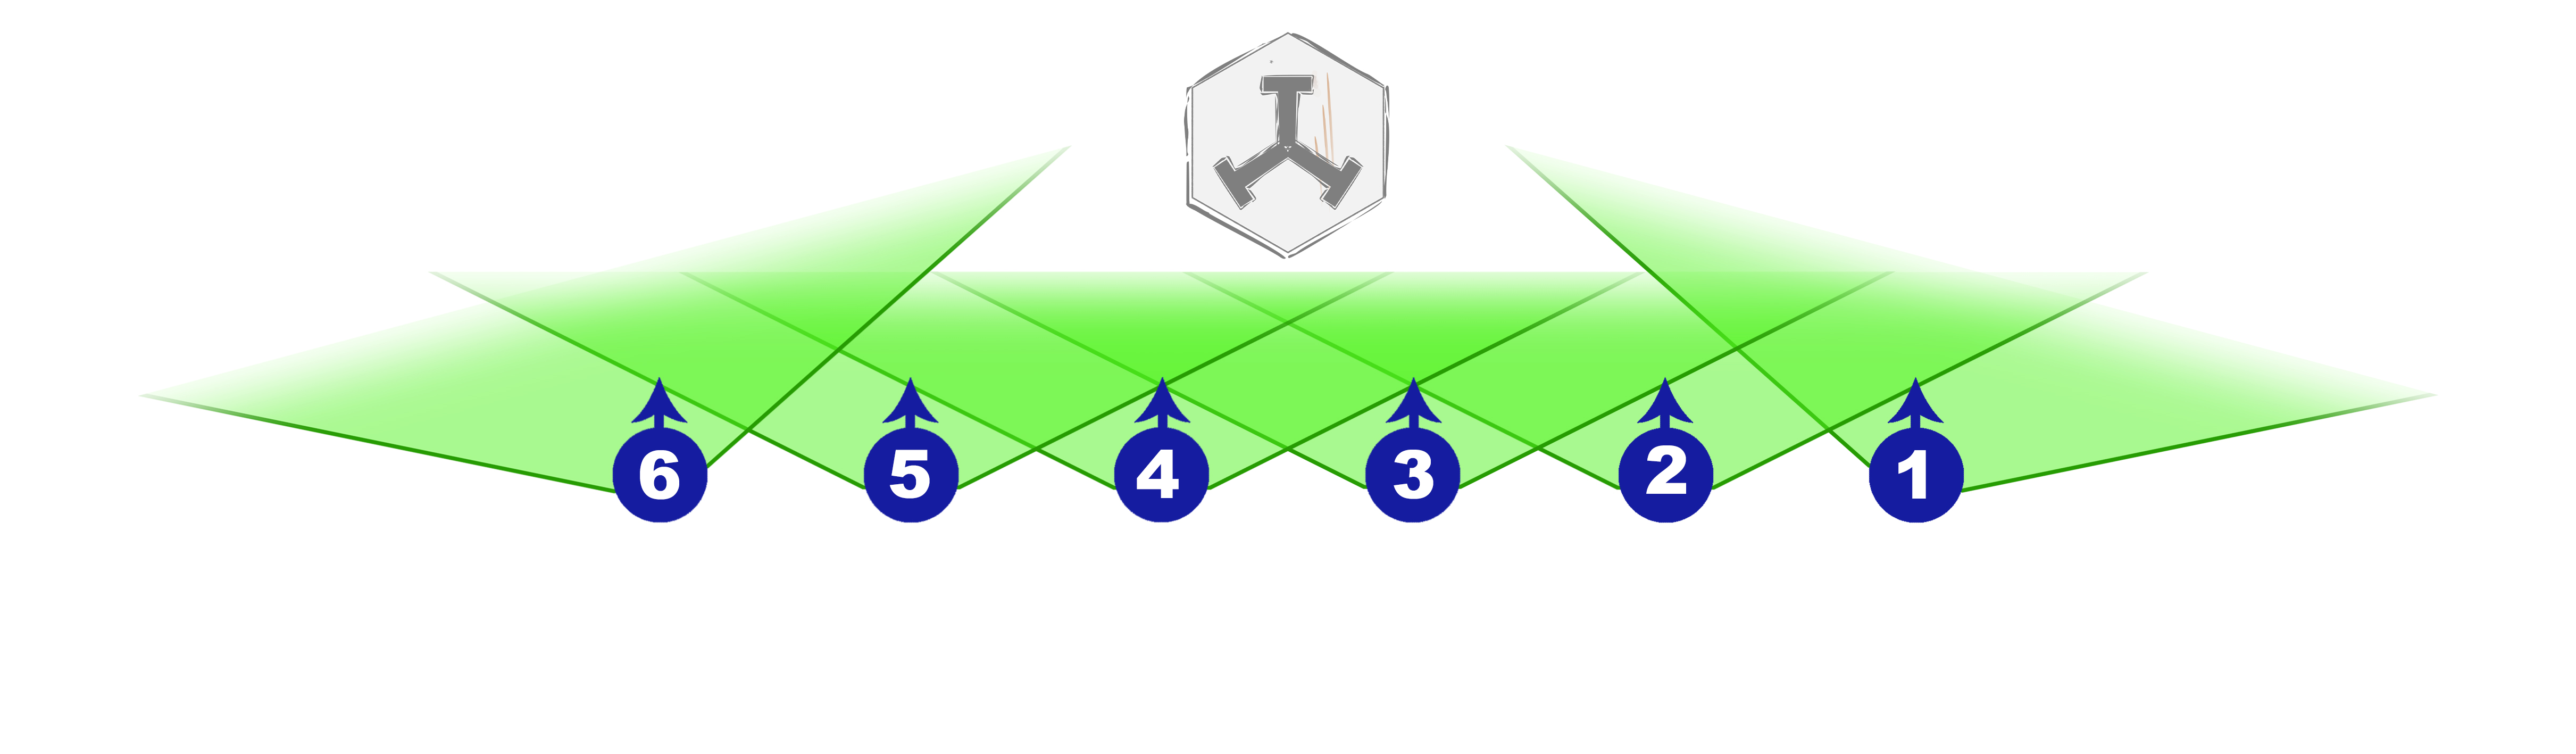
\includegraphics[width=0.95\linewidth]{./img/grundlagen/formationen/kette_6mann}
		\caption{Schützenkette}
\end{figure}